\documentclass[11pt, oneside, titlepage]{article}   	% use "amsart" instead of "article" for AMSLaTeX format
\usepackage[left=2.5cm,right=2.5cm,top=2.5cm,bottom=2.5cm]{geometry}
\usepackage[latin1]{inputenc}
\geometry{letterpaper}                   		% ... or a4paper or a5paper or ... 
%\usepackage[parfill]{parskip}    			% Activate to begin paragraphs with an empty line rather than an indent
\usepackage{graphicx}				% Use pdf, png, jpg, or eps§ with pdflatex; use eps in DVI mode
								% TeX will automatically convert eps --> pdf in pdflatex		
\usepackage[nottoc, section, numbib]{tocbibind}				% Add bibliography to table of contents
\usepackage{amssymb}
\usepackage{amsmath}				% Math fonts
\usepackage{mathtools}				% Enable \coloneqq for := operator
\usepackage{hyperref}				% Enable links (especially for table of contents)
\usepackage[margin=1cm]{caption}		% Set figure caption margins
\usepackage{subfig}					% Enable subfloats
\usepackage{multicol} 				% Enable multi columns
\usepackage{setspace}				% Enable set stretch
\hypersetup{						% Set link colors
    colorlinks,
    citecolor=black,
    filecolor=black,
    linkcolor=black,
    urlcolor=black
}
%SetFonts


\renewcommand*\contentsname{Table of Contents}	% Change name of table of contents
\renewcommand{\refname}{References}			% Change name of bibliography


% Title Page
\title{\bsc{Predicting Goals of Crowdfunding Campaigns}}
\author{Victor \bsc{Kristof}}
\date{Fall 2015}
%\pagestyle{headings}

\begin{document}
{\normalsize
\begin{multicols}{2}
\noindent �cole Polytechnique F�d�rale de Lausanne \\ LCA 3/4 \\ Semester Project \\ Fall Semester 2015�
\begin{flushright}
{
\includegraphics[scale = 0.75]{img/epfl_logo.pdf}} \\
\end{flushright}
\end{multicols}
}

\vspace{3cm}

\begin{center}
\thispagestyle{empty}
\setstretch{2.0}
{\Huge\bf  Predicting Goals of Crowdfunding Campaigns} \\
\vspace{2cm}
{\Large\bf
Semester Project
}
\vspace{2.0cm}

\setstretch{1.5}
\textbf{Victor Kristof} \\
Fall Semester 2015 \\
EDIC \\
\href{mailto:victor.kristof@epfl.ch}{victor.kristof@epfl.ch} \\

\vspace{2.0cm}
\date{}

\setstretch{1.0}
\vfill
\hfill
{\normalsize
\begin{multicols}{2}
\begin{flushleft}
Joint work with: \\
\textbf{Vincent Etter} \\
\textbf{Mohammad Emtiyaz Khan} \\
\end{flushleft}

\begin{flushright}
Supervisors: \\
\textbf{Patrick Thiran} \\
\textbf{Matthias Grossglauser} \\
\end{flushright}

\end{multicols}
}

\end{center}
%
%\title{Predicting Goals of Crowdfunding Campaigns}
%\author{Victor Kristof, Vincent Etter, Mohammad Emtiyaz Khan\\Matthias Grossglauser, Patrick Thiran}
%\date{\today}								% Activate to display a given date or no date
%
%\begin{document}
    %\maketitle
    \newpage
    \newgeometry{margin=3cm}
    \tableofcontents
    \newpage
%    \section{Introduction}
%        \subsection{Notations}
%        
%            \begin{itemize}
%                \item Let us denote $\mathbf{v}_{i:j}$, $i < j$ the subvector $\mathbf{u} = [v_i, ..., v_j]^\text{T}$ consisting of the elements $v_i$ to $v_j$ of the vector $\mathbf{v}$.
%                %\item Let us denote $(v_{i:j}, i \leq j)$ the subsequence $(u_n, n = i, ..., j) = (v_i, ..., v_j)$ consisting of the elements $v_i$ to $v_j$ of the sequence $(v_n, n = 1, ..., N)$.
%            \end{itemize}
   
   \section{Abstract} 
   In this document, we report our work on the prediction of goals of crowdfunding campaigns. We aim to improve the results obtained by Etter \cite{etter2013cosn} and used in Sidekick\footnote{\href{http://sidekick.epfl.ch}{http://sidekick.epfl.ch}}, where a probability of success is obtained in order to predict the outcome of the campaigns. The performances in their case was accurate very early in the time span of the campaigns, but only the success or failure was predicted. In this project, we first try to obtain a better classification accuracy and, then, we try to predict the final amount of pledged money for a given project. This information is more valuable to investors and creators, as they could obtain projections of the expected money that will be raised in the end. We therefore pose the problem as a regression problem and we investigate several techniques to solve it. First, we use gaussian processes, a powerful and flexible probabilistic modeling framework and, then, we experiment with mixture models. Better results are not achieved yet by lack of time, but interesting results have been found in the more complex context of predicting the final amount of pledged money. 
   
   This document is composed as follows. In Section \ref{sec:gp}, we provide a preview of the gaussian process framework for regression. In Section \ref{sec:problems}, we describe the models and results of our research to obtain satisfying results. Finally, in Section \ref{sec:future_work}, we give possible interesting directions to be followed in the future.  
   
   \section{Gaussian Processes}
   \label{sec:gp}
    Gaussian processes (GP) offer a powerful and flexible framework to perform regression. It allows to obtain a predictive distribution whose mean gives a point-wise prediction and predictive covariance variance provides a measure of uncertainty of the predictions. Through the definition of kernel in the covariance function, non-linearity and non-stationarity can be easily modeled. Finally, the kernels and the hyperparameters value have a great interpretability, which allows to explain more consistently the results and the data. Formally, as stated by Rasmussen and Williams \cite{Rasmussen:2005:GPM:1162254}, a gaussian process is a collection of random variables, any finite number of which have a joint gaussian distribution. It is completely specified by its mean function $m(\mathbf{x})$ and covariance function $k(\mathbf{x}, \mathbf{x'})$. It describes a distribution over functions and is noted 
    
    \begin{equation}
    \label{eq:gp}
    f(\mathbf{x}) \sim GP \left( m(\mathbf{x}), k(\mathbf{x}, \mathbf{x}') \right). 
    \end{equation}
    
    The important observation is that the joint distribution of the observed values $\mathbf{y}$ at inputs $X$ and new values $\mathbf{f}_*$ at new inputs $X_*$ is given by
    
    \begin{equation}
    \begin{bmatrix}
  \mathbf{y} \\
  \mathbf{f}_*
\end{bmatrix}
\sim 
\mathcal{N} \left( \mathbf{0},
\begin{bmatrix}
  K(X, X) + \sigma_n^2I & K(X, X_*) \\
  K(X_*, X) & K(X_*, X_*)
\end{bmatrix}
\right).
    \end{equation}
     
     We are actually interested by the new values $\mathbf{f}_*$, whose conditional distribution on the observations and inputs is
     
    \begin{eqnarray}
\mathbf{f}_* \mid X, \mathbf{y}, X_* &\sim& \mathcal{N}\left(\overline{\mathbf{f}}_*, \text{ cov}(\mathbf{f}_*)  \right) \label{eq:gp_predictive_distribution}\\
\overline{\mathbf{f}}_* &=& K(X_*, X) \left[ K(X, X) + \sigma_n^2I \right]^{-1}\mathbf{y} \label{eq:gp_predictive_mean} \\
\text{cov}(\mathbf{f}_*) &=& K(X_*, X_*) - K(X_*, X)\left[ K(X, X) + \sigma_n^2I \right]^{-1}K(X, X_*) \label{eq:gp_covariance}.
\end{eqnarray}
     
     Equation \ref{eq:gp_predictive_distribution} gives a predictive (gaussian) distribution whose predictive mean is given by Equation \ref{eq:gp_predictive_mean} and its corresponding predictive covariance is given by Equation \ref{eq:gp_covariance}. Informally, conditioning on $X$ and $\mathbf{y}$ means that we keep only the functions drawn from Equation \ref{eq:gp} that go through these observations. we can obtain predictions at any input $X_*$ while quantifying the uncertainty of our predictions. Then, conditioning on $X_*$ allows to obtain new values $\mathbf{f}_*$ at these points. The main drawback of this framework is the matrix inversion as it depends on the inputs $X$ of size $(N \times D)$ and that such operation is performed in time $O(N^3)$.
    
    \section{Problems Definition}
    \label{sec:problems}
    
	\subsection{Single-Project Regression}
        
		\subsubsection*{Model}
             
                    We are first approaching the problem as time series regression, considering only one project at a time. Our data set $\mathcal{D} = \left\{ (x_i, y_i) \mid i = 1, ..., T \right\}$ consists of $T$ observations, with $x_i$ the time index corresponding to an amount of pledged money $y_i$. Hence, we have $X = [1, ..., T]^\text{T}$, a vector of time indices, and $\mathbf{y} = [y_1, ..., y_T]^\text{T}$, a vector of observed values. We model the pledged money $f(X)$ at time indices $X$ as a gaussian process:
                    
                    \begin{equation}
                    		f(X) \sim GP \left( m(X), k(X, X') \right). 
                    \end{equation}
                    
                    Our goal is to predict the future values of the pledged money $\mathbf{f}_{t:T} = f(X_{t:T})$ at future time indices $X_{t:T} = [t, ..., T]^\text{T}$ after observing the values $\mathbf{y}_{1:t} = [y_1, ..., y_t]^\text{T}$ at time indices $X_{1:t} = [1, ..., t]^\text{T}$. In the GP framework, we can compute this prediction using
                    
                    \begin{eqnarray}
            			\mathbf{f}_{t:T}  \mid X_{1:t}, \mathbf{y}_{1:t}, X_{t:T} 	& \sim & 	\mathcal{N}\left(\overline{\mathbf{f}}_{t:T}, \text{ cov}(\mathbf{f}_{t:T})  \right) \\ 
           			\overline{\mathbf{f}}_{t:T}							& = & 	K(X_{t:T}, X_{1:t}) \left[ K_{1:t} + \sigma_n^2I \right]^{-1}\mathbf{y}_{1:t} \label{eq:predictive_mean} \\
           			\text{cov}(\mathbf{f}_{t:T}) 						& = & 	K_{t:T} - K(X_{t:T}, X_{1:t})\left[ K_{1:t} + \sigma_n^2I \right]^{-1}K(X_{1:t}, X_{t:T}) \label{eq:predictive_variance},
                    \end{eqnarray}
                    
                    with $K_{1:t} \coloneqq K(X_{1:t}, X_{1:t})$ and $K_{t:T} \coloneqq K(X_{t:T}, X_{t:T})$. Finally, the model's optimal hyperparameters $\theta_*$ are learned by maximizing the \textit{log marginal likelihood} over the first $t$ observed values:
                    
                    \begin{eqnarray}
                    		\theta_* 	&=& \underset{\theta} {\arg\max} \log p(\mathbf{y_{1:t}} \mid X_{1:t}, \theta) \\
    						&=& \underset{\theta} {\arg\max} \left\{ -\frac{1}{2}\mathbf{y}_{1:t}^\text{T} \left[ K_{1:t}+ \sigma_n^2I \right]^{-1}\mathbf{y}_{1:t} -\frac{1}{2}\log det\left[K_{1:t}+ \sigma_n^2I\right] -\frac{t}{2}\log 2\pi \right\} \label{eq:arg_max_log_marginal_likelihood}.
                    \end{eqnarray}
                                                   
		\subsubsection*{Results}
            		The major problem in this context is that the predictive mean $\mathbf{f}_*$ always falls back to the mean $m(\mathbf{x})$ very quickly. One solution is to sum two squared-exponential kernels and initializing one of them to a large length-scale in order to capture the global trend. This yields to some reasonable results for a few time steps after the last observation, but again falls back to the mean before reaching the end of the campaign, as displayed in Figure \ref{single_project_prediction}. Moreover, when using a model trained on one project to predict the future values of another one gives very poor performances.
		
			\begin{figure}[h]
                        		\begin{center}
                        			\includegraphics[scale=0.5]{img/single_project_prediction.pdf}
                        			\caption{Prediction (orange crosses) for a single project. Training is performed using the samples up to time 700 (black crosses). The actual trajectory is represented by the gray crosses. The blue line is the predictive mean and the light blue shade is the predictive variance. We see that the prediction is quite good for approximately 100 time steps, but it falls back to the mean (0) before the end of the campaign.}
                       		 	\label{single_project_prediction}
                       	 	\end{center}
                        	\end{figure}
           
         \subsection{Multi-Project Regression}
         	\subsubsection*{Model}
        			Our next idea is to consider $P$ projects together and try to learn the hyperparameters $\theta$ over various time series at the same time. In this case, for a given project $p$, we have a dataset $\mathcal{D}^{(p)} = \left\{ (x_i^{(p)}, y_i^{(p)}) \mid i = 1, ..., T \right\}$. Again, $y_i^{(p)}$ is the amount of pledged money at each time index $x_i^{(p)}$. Note that we have $x_i^{(p)}= x_i = i$, for all $p=1,...,P$ and all $i=1,...,T$. We combine the projects together to obtain the full dataset $\mathcal{D} = \left\{ \mathcal{D}^{(p)} \mid p = 1, ..., P \right\}$ (\textit{multi-task learning}). We then have the input $X = [1, ..., T]^\text{T}$, a vector of time indices, and the output $Y = \left[\mathbf{y}^{(p)} \right]_{p=1}^P$, a $(T \times P)$ matrix of observed values per project. For a given project $p$, we are trying to predict the pledged money $\mathbf{f}_{t:T}^{(p)} = f(X_{t:T}^{(p)})$ at future time indices $X_{t:T}^{(p)} = [t,...,T]^\text{T}$ after observing the values $\mathbf{y}_{1:t}^{(p)}$ at time indices $X_{1:t}^{(p)} = [1, ..., t]^\text{T}$. To do so in the GP framework, we have
        
                        \begin{equation}
                        		\mathbf{f}_{t:T}^{(p)} \mid X_{1:t}^{(p)}, \mathbf{y}_{1:t}^{(p)}, X_{t:T}^{(p)} \sim \mathcal{N} \left( \overline{\mathbf{f}}_{t:T}^{(p)}, \text{ cov}(\mathbf{f}_{t:T}^{(p)}) \right),
                		\end{equation}
                		        
                        with $\overline{\mathbf{f}}_{t:T}^{(p)}  $ and $\text{cov}(\mathbf{f}_{t:T}^{(p)}) $ obtained similarly to Equations \ref{eq:predictive_mean} and \ref{eq:predictive_variance}. The model's optimal hyperparameters $\theta_*$ are learned similarly to Equation \ref{eq:arg_max_log_marginal_likelihood} by maximizing the log marginal likelihood over all the projects, that is
                        
                        \begin{equation}
                        		\theta_* = \underset{\theta} {\arg\max} \sum_{p=1}^P \log p(\mathbf{y}^{(p)} \mid X^{(p)}, \theta).
                        \end{equation}
                        
                        Note that during training, we consider the ``full" projects, that is $\mathbf{y}^{(p)} = \mathbf{y}_{1:T}^{(p)}$ and $X^{(p)} = X_{1:T}^{(p)}$.
                        
         	\subsubsection*{Results}
        			Again, we couldn't obtain good results with this approach, as the predictions always fall back very quickly to the mean of the GP. We run the following experiment. We consider 1000 projects. We take 800 of them to learn the hyperparameters and 200 as test set. For each new project, we observe 1 to $t$ points and try to predict the final amount of pledged money. We increase $t$ from 1 to 1000 by increment of 50 time steps. The learning curve is displayed in Figure \ref{fig:multiproject_prediction}. As we see, we obtain 50\% of accuracy. It happens that the model always predict 0, that is a failure, and since we have approximately the same number of successful and failed projects, we obtain half of them correctly.
			
			\begin{figure}[h]
                        		\begin{center}
                        			\includegraphics[scale=0.5]{img/multiproject_prediction.pdf}
                        			\caption{The 50\% accuracy obtained here is due to the fact that the last time step (end of the campaign) is always predicted to be 0, which corresponds to a failure. Since half of the projects are successful and the other half are failed, the accuracy is 50\%. }
                       		 	\label{fig:multiproject_prediction}
                       	 	\end{center}
                        	\end{figure}			 
        
         \subsection{Project Classification}
         	\subsubsection*{Model}
            		We then decide to perform a simpler task. Instead of trying to predict future amounts of pledged money after some observations, we try now to classify whether a project $p$ will be successful ($c^{(p)} = 1$) or not ($c^{(p)} = 0$). Indeed, by separating the data set into two classes (\textit{successful} and \textit{failed}), we notice that they have a very different profiles, as shown in Figure \ref{fig:two_profiles}, and therefore should be easy to discriminate. To do so, we train one GP using the successful projects and one using the failed projects. We then try to determine whether a new, partially observed project will be successful or not. 
			\begin{figure}[h]
                        		\begin{center}
                        			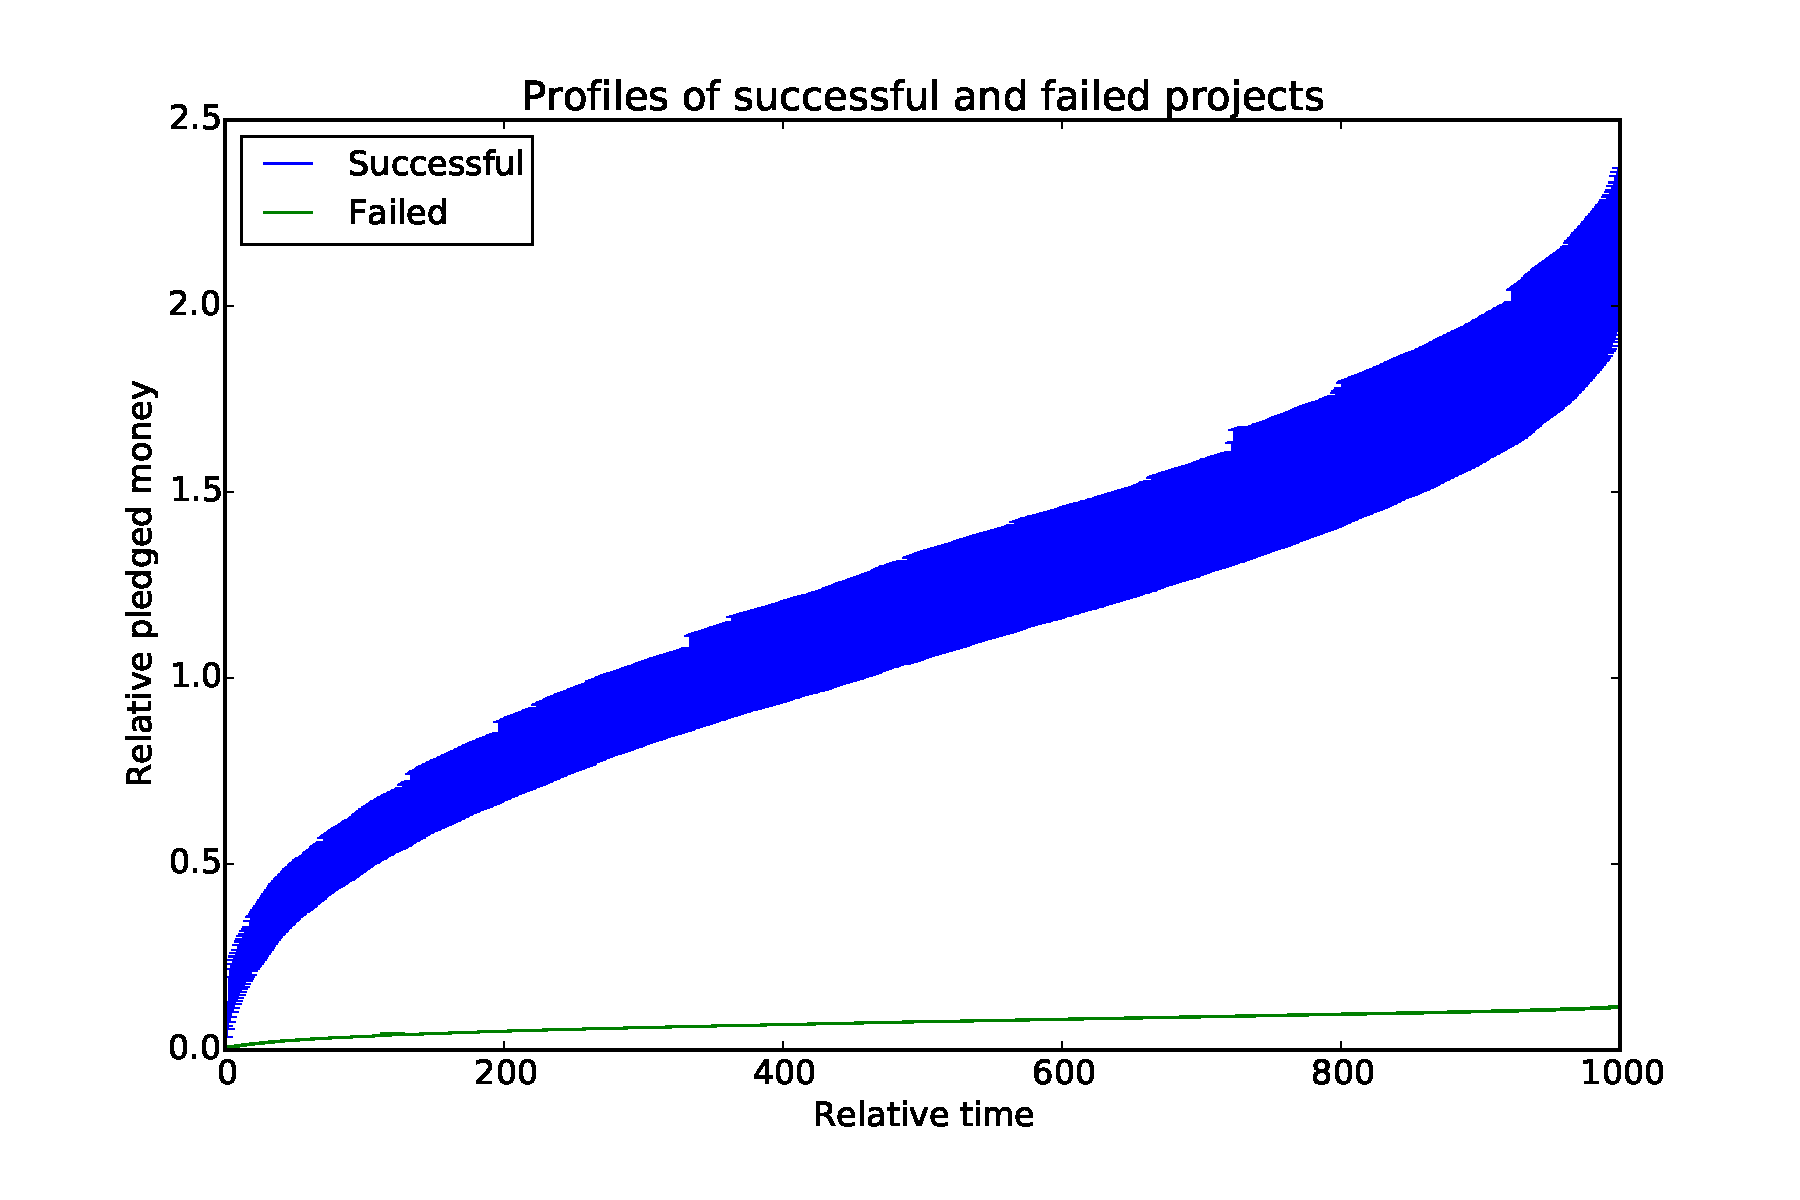
\includegraphics[scale=0.5]{img/two_profiles.pdf}
                        			\caption{Average trajectory and standard error for both classes displaying two very distinct profiles that suppose the possibility to classify the projects.}
                       		 	\label{fig:two_profiles}
                       	 	\end{center}
                        	\end{figure}
			We learn $\theta_s$ the hyperparameters of a GP over $P_s$ successful projects  and $\theta_f$ the hyperparameters of a GP over the $P_f$ failed projects. That is, we obtain the two sets of hyperparameters by maximizing the log marginal likelihoods
        
                        \[\theta_s = \underset{\theta} {\arg\max} \sum_{p=1}^{P_s} \log p(\mathbf{y}_s^{(p)} \mid X^{(p)}, \theta)\]
                        \[\theta_f = \underset{\theta} {\arg\max} \sum_{p=1}^{P_f} \log p(\mathbf{y}_f^{(p)} \mid X^{(p)}, \theta),\]
                        
                        where $\mathbf{y}_s$ and $\mathbf{y}_f$ denote the observations of the successful and failed projects respectively. We then determine the success state $c^{(p)}$ of a new project $p$ with partial observations $\mathbf{y}_{1:t}^{(p)}$ as
                        
                        \[c^{(p)} = 
                        \begin{cases}
                            1, & \text{ if } \log p(\mathbf{y}_{1:t}^{(p)} \mid X_{1:t}^{(p)}, \theta_s) > \log p(\mathbf{y}_{1:t}^{(p)} \mid X_{1:t}^{(p)}, \theta_f) \\
                            0, & \text{ otherwise }
                        \end{cases}.\]
            
         	\subsubsection*{Results}
		Similarly to the multi-project regression, the same class is always predicted. Therefore, an accuracy of 50\% is achieved in this case as well. However, the trajectories shown in Figure \ref{fig:two_profiles} suggest that classification should possible and, hence, the hyperparameters of the GP's are probably not well learned.
        
         \subsection{Output as Input}
         \label{sec:output_input}
         	\subsubsection*{Model}
        			We change completely the set up. Instead of using the time as input and trying to predict the pledged money at new time indices, we now consider the pledged money at each time step as input and the last time index as the output. That is, we have now a dataset $\mathcal{D} = \left\{ (\mathbf{x}^{(p)}, y^{(p)}) \mid p = 1, ..., P \right\}$ with $\mathbf{x}^{(p)} = \mathbf{y}_{1:t}^{(p)}$ and $\mathbf{y}^{(p)} = y_T^{(p)}$. We then have $X = \left[\mathbf{x}^{(p)}\right]_{p=1}^P$, a $(P \times t)$ matrix of pledged money, and $\mathbf{y} = \left[y_T^{(p)}\right]_{p=1}^P$, a vector corresponding to the total amount of money at the end of the $P$ campaigns. The difference with the previous approach is that now the features for each project are the amount of pledged money at different time steps and not the same (shared) input values $[1,...,T]^\text{T}$. Note that $t$ can be arbitrarily set to any value up to $T$ and that the number of samples taken in $[1, t]$ (the \textit{granularity}) can also be determined arbitrarily. We display an example of three different features in Figure \ref{fig:input_output_global}. The projects above $y=1$ are the successful projects. The projects on the right side of $x=1$ are projects which reached their goal at the time corresponding to the feature. As the projects approach their end, the amount of money becomes linear. Indeed, the amount they have near the end is often the money the have at the end. Note the horizontal cluster at $y=1$ in the third plot. We see that a lot of projects reach their goal in the last moments of their campaigns. Also, we notice that successful projects are all ``over the place", whereas the failed ones are confined to the left hand of the space.  
        			\begin{figure}[h]
                        		\begin{center}
                        			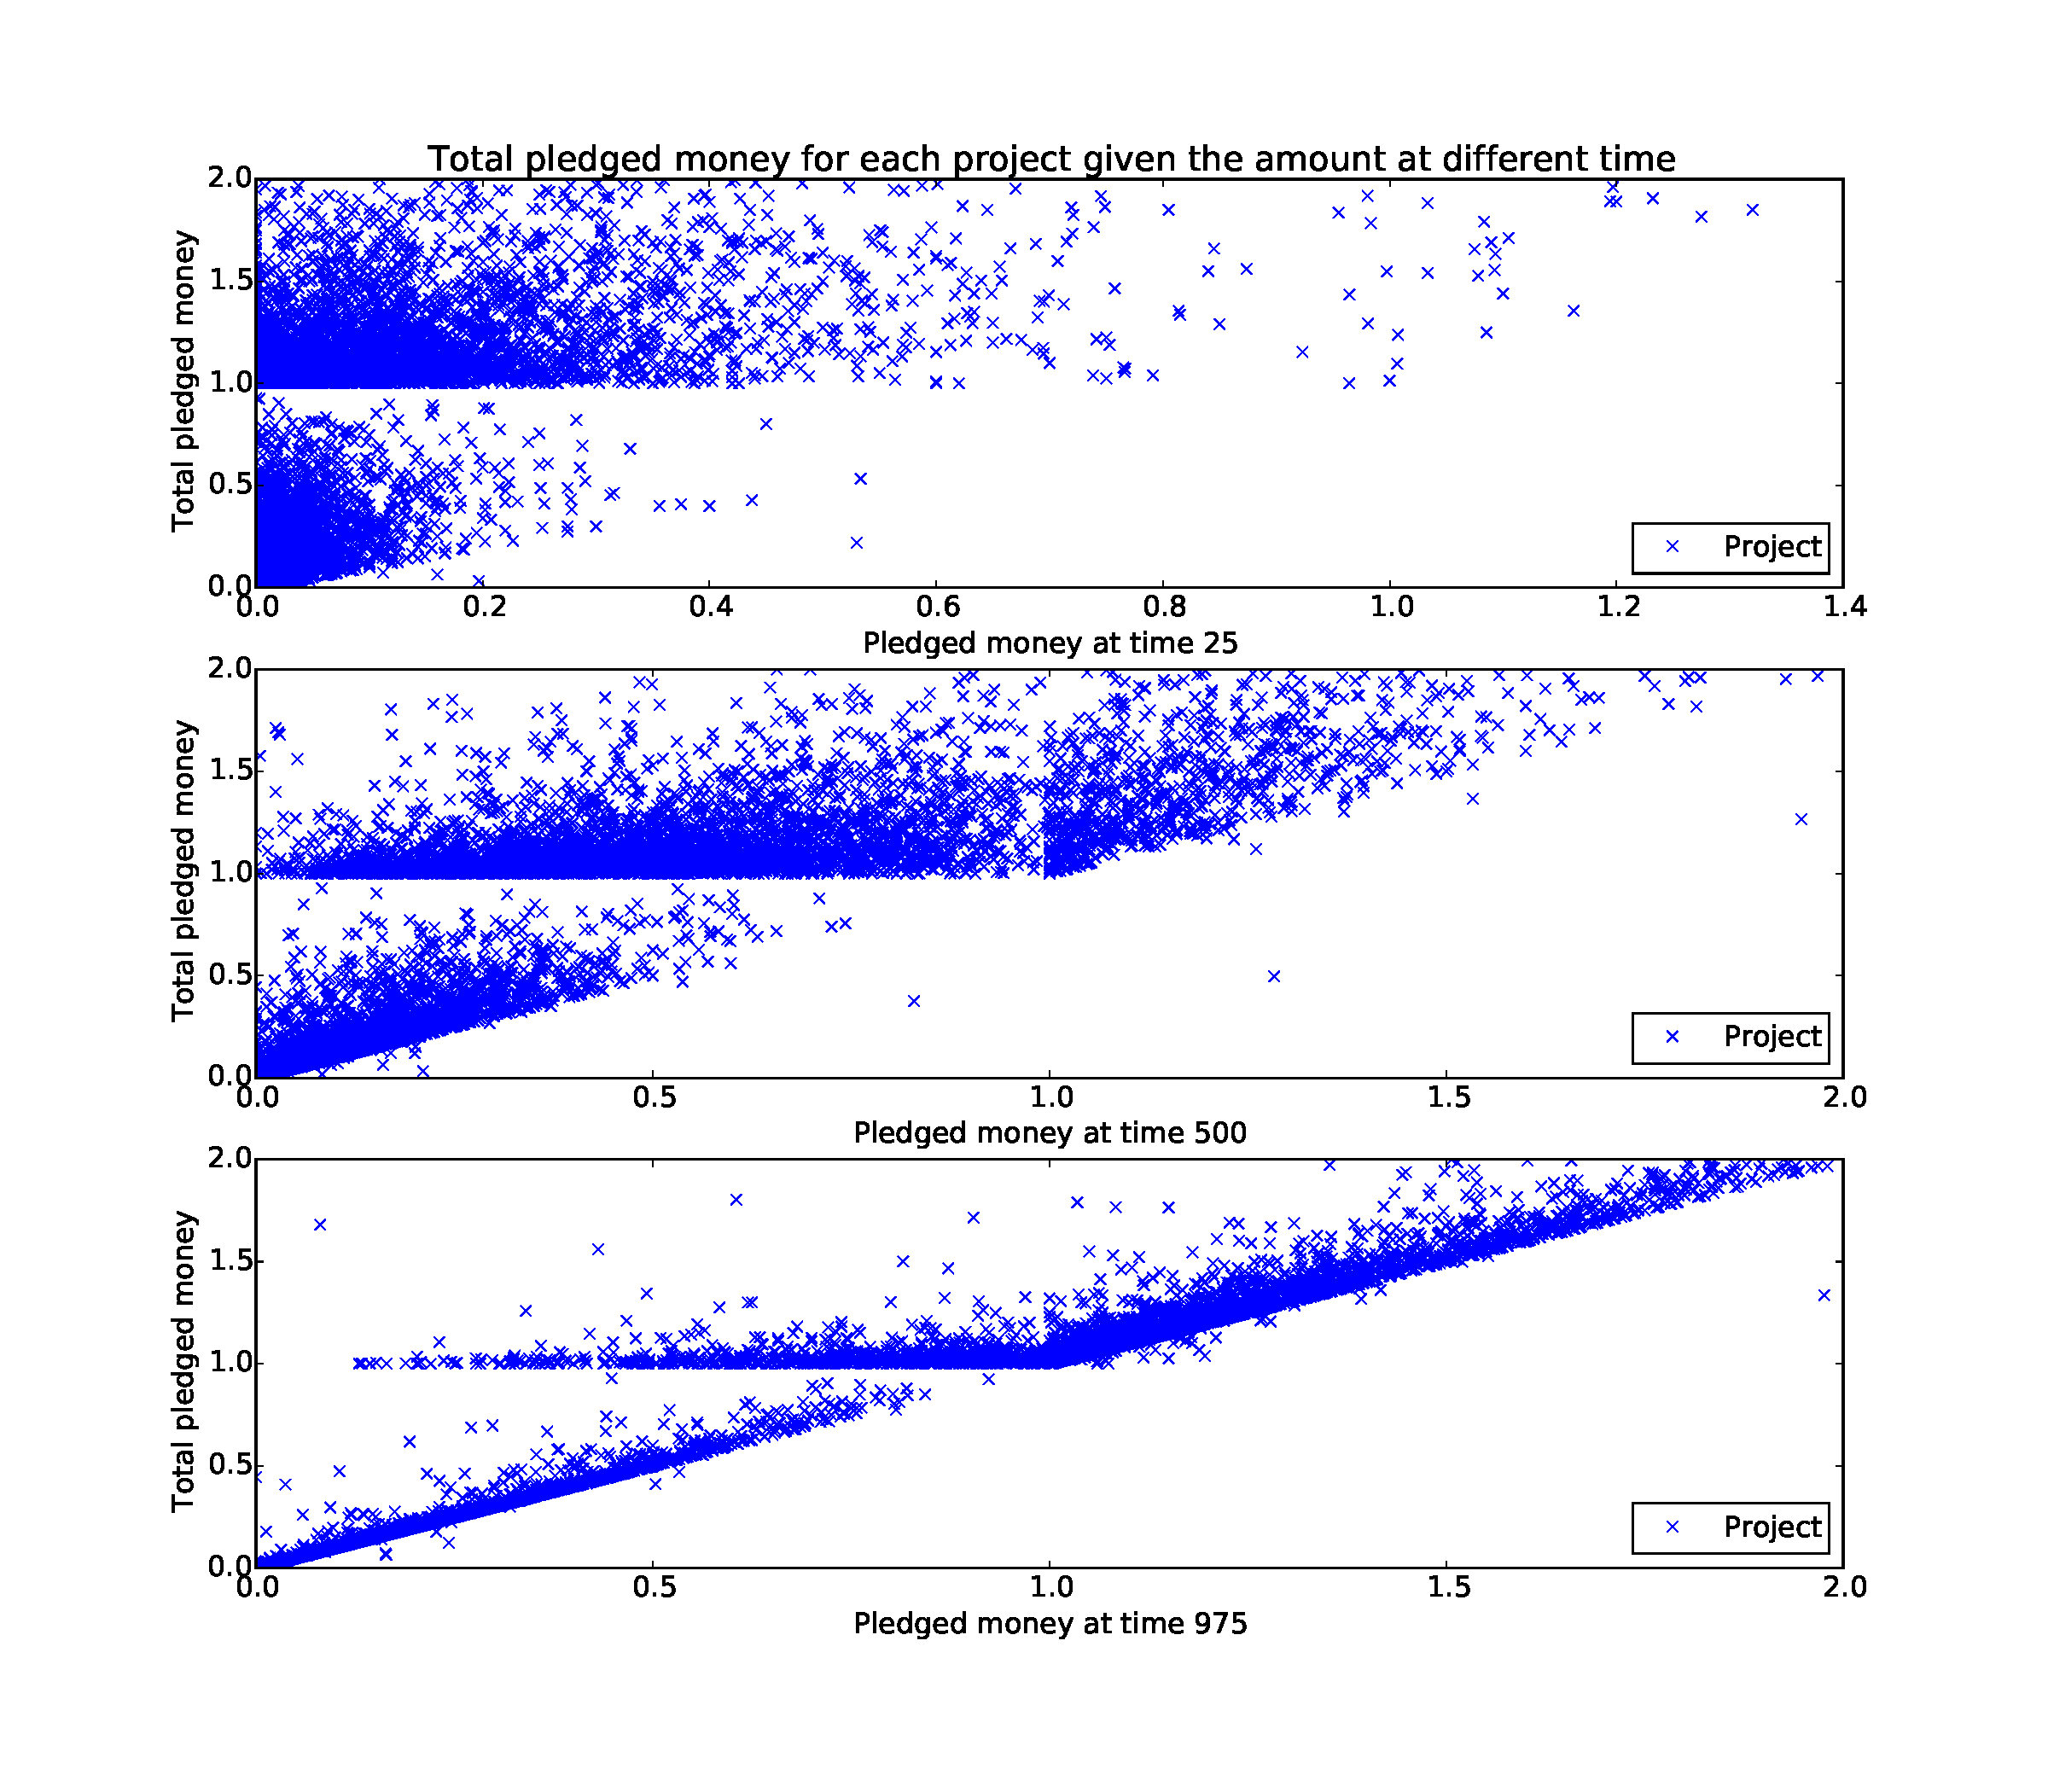
\includegraphics[scale=0.4]{img/input_output_global.pdf}
                        			\caption{Final pledged money (y-axis) for each project versus the amount they had at time 25 (early in the campaign), 500 (middle of the campaign) and 975 (near the end of the campaign). As the projects approach their end, the amount of money becomes linear. Indeed, the amount they have near the end is often the money the have at the end. Note the horizontal cluster at $y=1$ in the third plot. We see that a lot of projects reach their goal in the last moments of their campaigns.}
                       		 	\label{fig:input_output_global}
                       	 	\end{center}
                        	\end{figure}
		
		Our goal now is to predict, for a new project $p$, the final amount of pledged money $y_T^{(p)} = f(\mathbf{y}_{1:t}^{(p)})$ given $\mathbf{y}_{1:t}^{(p)}$ the money received up to time $t$ after observing the total pledged money for all projects $\mathbf{y} = \left[y_T^{(p)}\right]_{p=1}^P$ and the money they received up to time $t$, $X = \left[ \mathbf{y}_{1:t}^{(p)} \right]_{p=1}^P$. In the GP framework, we can compute this prediction using
        			 
			 \begin{eqnarray}
			 	y_T^{(p)} \mid X, \mathbf{y}, \mathbf{y}_{1:t}^{(p)} 	& \sim & 	\mathcal{N}\left(\overline{y}_T^{(p)}, \text{ cov}(y_T^{(p)})  \right) \\
                            	\overline{y}_T^{(p)}							& = &	K(\mathbf{y}_{1:t}^{(p)}, X) \left[ K(X, X) + \sigma_n^2I \right]^{-1}\mathbf{y} \\
                            	 \text{cov}(y_T^{(p)}) 						& = & 	K(\mathbf{y}_{1:t}^{(p)}, \mathbf{y}_{1:t}^{(p)}) - K(\mathbf{y}_{1:t}^{(p)}, X)\left[ K(X, X) + \sigma_n^2I \right]^{-1}K(X, \mathbf{y}_{1:t}^{(p)}).
                            \end{eqnarray} 
        		A point-wise prediction of the final amount of money for a project $p$ is given by $\overline{y}_T^{(p)}$. We can furthermore classify the project as successful if $\overline{y}_T^{(p)} \geq 1$ and failed otherwise.
		 
        		\subsubsection*{Results}
         	\label{sec:output_input_results}
        		We run the following experiment. Using the above data set, we train a GP on $t=25, 50, ..., 975$ on 70\% of the data and compute the accuracy and the RMSE of the last 30\% of the data. We remove projects that obtain more that $M=2$, 10 and 20 times their goal (we call these \textit{outliers}). We repeat the procedure 10 times with 10 randomly chosen splits of the data set and we take the median accuracy and RMSE across the 10 runs at each $t$. The results are displayed in Figure \ref{fig:gp_results}.
		\begin{figure}[h!]
                    	\centering
                    	\begin{tabular}{c}
                    		\subfloat[Accuracy.]{\includegraphics[scale=.55]{img/accuracy_final_gp.pdf}} \\
                    		\subfloat[RMSE.]{\includegraphics[scale=.55]{img/rmse_final_gp.pdf}}
                    	\end{tabular}
                    	\caption{Results obtained for three thresholds of outliers and using one gaussian process.}
                    	\label{fig:gp_results}
                    \end{figure}

		Note that the data set consists of 1000 projects only, as training a gaussian process on the 16000 projects (or even 5000) is unfeasible on a single computer without using variational inference. The results are below the baseline established by the best predictor of Etter \cite{etter2013cosn}, but we obtain also a prediction of the final amount of money and we only use one money-based feature. We also show in Figure \ref{fig:gp_output_input} an example of the fit by a gaussian process at an early stage of the campaigns. We see that the two modes are not very well captured by only one regression, which explains the not so good performance. Our next step is therefore to use a mixture model in order to improve our results by capturing the different trends.
		\begin{figure}[h!]
                        		\begin{center}
                        			\includegraphics[scale=0.5]{img/gp_output_input.pdf}
                        			\caption{A gaussian process fit on 1000 projects at time 25 (early in the campaign). The regression does not represent very well }
                       		 	\label{fig:gp_output_input}
                       	 	\end{center}
                        	\end{figure}
	
         \subsection{Mixture of Linear Regressions}
         \label{sec:mlr}
         	\subsubsection*{Model}
		We start by using a mixture of linear regressions in order to see is we can actually fit different trends in the data and to establish a baseline for the mixture models. The model that we use to obtain a prediction for the final amount of pledged money $y_p$ for a project $p$ given the previous observed money $\mathbf{x}_p$ is 
		\begin{equation}
			p(y_p \mid \mathbf{x}_p, \mathbf{\theta}) = \sum_{k=1}^K \pi_k \mathcal{N}(y_p \mid \mathbf{\beta}_k^{\text{T}}\mathbf{x}_p, \sigma_k^2).
		\end{equation}
		The parameters $\mathbf{\theta} = \left\{ \pi_k, \mathbf{\beta}_k, \sigma_k^2 \right\}_{k=1}^K$ are learned using an EM algorithm, as described in Bishop \cite{Bishop:2006:PRM:1162264}. We therefore learn a predictive distribution. The point-wise prediction of the final amount of pledged money is obtained by computing the mean of this distribution, that is
		\begin{eqnarray}
			y_p^* &=& \mathbb{E}\left[p(y_p \mid \mathbf{x}_p, \mathbf{\theta})\right] \nonumber \\ 
				 &=& \sum_{k=1}^K \pi_k \mathbb{E}\left[\mathcal{N}(y_p \mid \mathbf{\beta}_k^{\text{T}}\mathbf{x}_p, \sigma_k^2)\right] \nonumber \\
				 &=& \sum_{k=1}^K \pi_k  \mathbf{\beta}_k^{\text{T}}\mathbf{x}_p.
		\end{eqnarray}
		
		Other ways of obtaining point-wise predictions should be also investigated, especially the median. However, in this case and as described later in this section, the predictive distribution is usually a gaussian (one of the $\pi_k$ is very big) and therefore the mean and the median are the same. Finally, as previously, we classify a project as successful if $y_p^* \geq 1$ and failed otherwise.
		
        		\subsubsection*{Results}    
		We show in Figure \ref{fig:weights_outlier_2} the fit of the mixture of linear regressions. We see that two trends are indeed learned at the beginning and at the end, even though in this latter case one of the two components has a large mixture weight and hence explains almost everything. At the middle, however, the two components converge and only one line is learned. 
		\begin{figure}[h]
                		\begin{center}
                			\includegraphics[scale=0.35]{img/weights_outlier_2.pdf}
                			\caption{Mixture of linear regressions at different times (early, middle and at the end of the campaigns).}
               		 	\label{fig:weights_outlier_2}
               	 	\end{center}
                	\end{figure}
	
		We run the same experiment as in Section \ref{sec:output_input_results}. The resulting accuracy and RMSE are displayed in Figure \ref{fig:mlr_results}. They are worse than the ones obtained using one gaussian process only. However, they are more consistent as we could use the whole data set to run the experiment. Moreover, the model is linear and therefore much simpler than the gaussian process. The two components give now a better explanation of the data and will be investigated more, as described in the next section. 
		\begin{figure}[h!]
                    	\centering
                    	\begin{tabular}{c}
                    		\subfloat[Accuracy.]{\includegraphics[scale=.55]{img/accuracy_final_mlr.pdf}} \\
                    		\subfloat[RMSE.]{\includegraphics[scale=.55]{img/rmse_final_mlr.pdf}}
                    	\end{tabular}
                    	\caption{Results obtained for three thresholds of outliers and using one gaussian process.}
                    	\label{fig:mlr_results}
                    \end{figure}
	
         %\subsection{Mixture of Gaussian Processes}
        % 	\subsubsection*{Model}
        %		\subsubsection*{Results}
		
	\subsection{Next Steps}
	In Sections \ref{sec:output_input} and \ref{sec:mlr}, only one feature was used in the models. The first improvement we will try is to increase the number of features in our mixture of linear regressions. This means that we need to find the optimal \textit{granularity} of the subsampling, as too many features might decrease the performances and too few features are not representative of the data. On the other hand, as we would like to be as accurate as possible as early as we can, we don't have a lot of room to vary the number of samples. For instance, at time 10 we have at most 10 features.
	
	Secondly, the number of mixture components can be arbitrarily set (we only tried with $K=2$ components). More components means that we can fit different trends in the data and potentially obtain better results. Also, by computing the posterior probability of each components given a new data point, we can give interesting information about the final amount of money a given project can collect. 
	
	Then, of course, we should improve on the linear model and use a non-linear one, like a mixture of gaussian processes for instance. This will enable much more flexibility in each of the components, while benefiting from the advantages of a mixture model as described above. The main challenge will reside in the training of the model using the full data set.
	
	We should also try to use non-normalized data. In fact, so far the projects are normalized with respect to their goal. This means that a project targeting \$3,000 and having collected half of it is considered the same as a project demanding \$1,000,000 and having collected \$500,000. Of course the magnitude of these two projects is not equivalent and hence we should use this knowledge. 
	
	Finally, outliers are currently arbitrarily discarded. We should in the end use some methods to handle these cases better, as simply ignoring them is to simplistic.
	
    \section{Future Work}
    \label{sec:future_work}
    Two possible paths should be considered once a useful model is found. The first one would be to study the evolution of the co-backer graph and the evolution of the pledged money jointly, as events in one process influence the other one. More concretely, this means that we should investigate joint probabilistic models of information diffusion and network evolution to model the joint dynamics of the system. Some work in this direction has been done in Farajtabar et al. \cite{DBLP:journals/corr/FarajtabarWGLZS15} and Jimenez Rezende et al. \cite{10.3389/fncom.2014.00038}. Unfortunately, Kickstarter doesn't display anymore the backers, which prevents the construction of the co-backer graph. We have it for the current data set however.
    
    The other problem that could be tackled is the one of project pricing. Indeed, it would be interesting to guess how much a project is worth and hence what would be the optimal goal that maximizes the probability of success. This problem is related to the one of product pricing in finance and economics (e.g. stock pricing or house pricing). In our case, however, we can extract more features, such as text-based features from the description of the project, or other meta-data, as the videos, images or who are the initiators of the project. 
	
	 \clearpage
	 
	\bibliographystyle{plain}
	\bibliography{bibliography}
    
\end{document}  